\documentclass[aspectratio=169,11pt]{beamer}
\usetheme{default}
\usecolortheme{seahorse}
\setbeamertemplate{navigation symbols}{}
\setbeamertemplate{footline}[frame number]
\setbeamertemplate{itemize items}[circle]
\usepackage{fontspec}
\usepackage{fancyvrb}
\setmonofont{DejaVu Sans Mono}[Scale=0.85]
\newcommand{\hl}[1]{\colorbox{yellow}{#1}}
\newcommand{\todo}[1]{{\color{red}\emph{#1}}}

\title{Rust codecs: streaming byte transformations}
\author{Oleg Parashchenko}
\date{November 2026}

\begin{document}
\begin{frame}\titlepage\end{frame}
\begin{frame}{Contents}\tableofcontents\end{frame}

\section{What's going on?}
\begin{frame}[fragile]{What's going on? Bytes in, transform, bytes out}
\newlength{\vw}\setlength{\vw}{0.52\textwidth}
\begin{minipage}[c]{\vw}
\mbox{\special{pdf:ann width \the\vw\space height \the\dimexpr0.4874\vw\relax\space << /Type /Annot /Subtype /Movie /Border [0 0 0] /T (rot13) /Movie << /F (rot13.mp4) /Aspect [597 291] /Poster true >> /A << /Start 0 /Mode /Repeat >> >>}%
  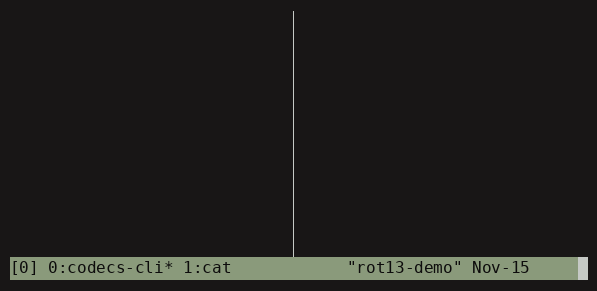
\includegraphics[width=\vw]{rot13_poster.png}%
  \sbox0{\fcolorbox{white}{black!70}{\color{white}\small\,{\fontspec{DejaVu Sans}\char"25B6}\ click to play\,}}%
  \hspace{-\vw}\makebox[\vw][c]{\raisebox{\dimexpr0.2437\vw-0.5\ht0-0.5\dp0\relax}{\usebox0}}}
\end{minipage}\hfill
\begin{minipage}[c]{0.44\textwidth}
\begin{Verbatim}[fontsize=\scriptsize,commandchars=\\\{\}]
let mut source = BufReadSource::new(
    io::stdin().lock(),
);
let mut sink = StdSink::new(
    io::stdout(), vec![0u8; 4096],
)?;
\hl{stream_to_stream}(
    &mut source, // Any Source
    \hl{rot13()},
    &mut sink, // Any Sink
)?;
\end{Verbatim}
\end{minipage}
\end{frame}

\section{Why codecs?}
\begin{frame}[fragile]{Why codecs? My use case}
Streaming JSON (crate \texttt{scan\_json}): process through a sliding window.

\medskip
\begin{Verbatim}[fontsize=\scriptsize]
{
  "image": "iVBORw0KGgoAAAANS...",
  "url":   "https%3A%2F%2Fexample.com%2Fpath",
  "text":  "Line 1\nLine 2\t\"quoted\""
}
\end{Verbatim}

\medskip
Streaming transformations are needed. A standard interface?
\end{frame}

\begin{frame}{Prior art}
ChatGPT research mode:
\begin{quote}\small
Rust has had many serious pieces of groundwork, but almost all of them
optimized either framing, compression, or format-specific ergonomics.

\medskip
A \hl{general} standard for stateful, composable, allocation-light streaming
byte rewriters \hl{remains a visible gap}.
\end{quote}
\medskip
Full report: \small\url{https://github.com/olpa/rust-codecs/blob/master/deep-research-report.md}
\end{frame}

\section{About the author}
\begin{frame}{About the author}
\textbf{Oleg Parashchenko}

\smallskip
\url{https://uucode.com/}\\
\url{https://github.com/olpa/}\\
\url{https://www.linkedin.com/in/olepar/}

\medskip
Background: Linux, system programming, math

\medskip
Quietly useful:
\begin{itemize}
\item bbAntiSpam
\item CALS tables for \LaTeX
\end{itemize}

\medskip
And now working on: Streaming JSON, codecs
\end{frame}

\section{About the talk}
\begin{frame}{About the talk}
\begin{itemize}
\item A design story, not an API reference
\item Three decisions you (and prior art) wouldn't predict:
  \begin{itemize}
  \item early stop
  \item full consume
  \item \texttt{Source}/\texttt{Sink}
  \end{itemize}
\item A glimpse at what else becomes possible
\end{itemize}
\end{frame}

\section{Requirements and the idea}
\begin{frame}[fragile]{First requirements and the idea}
Requirements:
\begin{enumerate}
\item streaming processing: bytes in, bytes out
\item zero cost for in-memory: no unneeded copies/movements for slice in, slice out
\item \dots{} to be continued
\end{enumerate}
First idea: two iterators
\begin{itemize}
\item Inner iterator, cheap, essentially scanning a memory
\end{itemize}
\begin{Verbatim}
while(*tgt++=*src++);
\end{Verbatim}
\begin{itemize}
\item Outer iterator: load/save a block of memory to an external storage
\end{itemize}
\end{frame}

\section{Prior art}
\begin{frame}{Prior art: shortlist}
\begin{itemize}
\item tokio codecs
\item compcol --- very close to what I want. Collection of compression algorithms.
\item Honorary mention: base64 algorithm as an ``adversarial'' use case
\end{itemize}
\end{frame}

\begin{frame}{Updated requirements}
\begin{enumerate}
\item streaming processing: bytes in, bytes out
\item zero cost for in-memory: no extra copies/movements for slice in, slice out
\item \todo{placeholder: find what's interesting in compcol}
\item \todo{placeholder: find what's interesting in tokio}
\item \todo{placeholder: find what's needed for base64}
\end{enumerate}
\end{frame}

\section{Compcol}
\begin{frame}{Compcol interface}
\begin{itemize}
\item Process step $\to$ \texttt{Progress}, \texttt{Status}
\item Code/decode
\item Slice to slice instead of an iterator: OK
\item flush, finish. Hello from base64, we'll come to it
\end{itemize}
\end{frame}

\begin{frame}{Compcol interface --- 2}
Result of a codec step.
\begin{itemize}
\item Codec-initiated end of the stream
\item There is also ``skip N bytes'', but for me it doesn't need a definition through the interface
\end{itemize}
\end{frame}

\begin{frame}{Requirements rewrite}
\begin{enumerate}
\item streaming processing
\item zero cost for in-memory
\item finish, maybe flush and in-band end
\end{enumerate}
\end{frame}

\begin{frame}{AI slop}
\begin{itemize}
\item I've never seen such unclear code.
\item Manual investigation: indeed, not so easy.
\item A corner case sits on a corner case and harnesses a corner case
\end{itemize}
\end{frame}

\section{Base64}
\begin{frame}{Base64}
\begin{itemize}
\item Blocks of 3 bytes $\to$ blocks of 4 bytes
\item Last block: with filling bytes (must do)
\end{itemize}
\end{frame}

\begin{frame}[fragile]{Base64 challenge}
Input: \texttt{[x][x][x][o][o]}\\
Output: \texttt{...}

\medskip
Convert:
\begin{itemize}
\item Can't proceed with input $\to$ 0 bytes
\item Can't proceed with output $\to$ 0 bytes
\end{itemize}
Step output:
\begin{Verbatim}
{
  consumed: 0;
  written: 0;
}
\end{Verbatim}
0/0: is the codec stalled? How to fix?
\end{frame}

\section{Solution}
\begin{frame}{Solution}
Consume full, or write full.

\medskip
The returning type: \todo{\dots}

\bigskip
\alert{A big insight.} If you take whatever with you, take this insight: a codec should do full.
\end{frame}

\begin{frame}{Final interface}
\todo{(to be filled)}
\end{frame}

\section{I/O backend}
\begin{frame}{I/O backend: Sources and Sinks}
\begin{itemize}
\item For zero overhead for in-memory: slices/Vecs
\item \todo{\dots interface \dots}
\item Differentiator from other codec stuff, which is tied to Reader, Writer and their async versions
\end{itemize}
\end{frame}

\section{Early stop}
\begin{frame}{Early stop}
\begin{itemize}
\item Codec: \texttt{ParseString}
\item Taken from the compression codecs (compcol)
\item New use case: parsing
\item Example: parse until a quote
\item \texttt{stream\_to\_stream}: getting tokens
\item But: \texttt{NullSink}, getting position $\to$ in-place parsing, no byte moving
\item In investigation, a topic for the next year
\end{itemize}
\end{frame}

\section{Inside}
\begin{frame}{Inside}
\begin{itemize}
\item \texttt{stream\_to\_stream}
\item Sink/Source and CodecReader/CodecWriter for \texttt{std::io} and \texttt{embedded\_io}
\item Async version later
\item Source for \texttt{u8} slice, Source/Sink for \texttt{u8} Vec
\end{itemize}
\end{frame}

\begin{frame}{Inside: codecs}
All codecs from ``compcol'' (lz, \dots), encoding-rs, slip, async-compression, bytes\_rw

\medskip
Provisional (mostly AI generated with review):
\begin{itemize}
\item base64
\item json encode and decode
\item TODO quoted-printable
\item TODO urlencode
\end{itemize}
\end{frame}

\section{Call for participation}
\begin{frame}{Call for participation: Codecs}
Create codecs:
\begin{itemize}
\item ``convert'' function
\item Inner staging to hold bytes when it can't produce reasonable output, but must consume full input
\end{itemize}
No need to care for I/O and UX, just convert.

\medskip
This is a mega-bonus: before, each transformation crate had to invent its own interface for bytes. No need for it anymore.

\medskip
Second insight from the talk: the byte pull-push got a new potential standard.

\medskip
\texttt{CREATING-CODECS.md}
\end{frame}

\begin{frame}{Call for participation: Parser combinators}
Nothing done by me yet, but the way is clear.
\end{frame}

\begin{frame}{Call for participation: I/O backends}
More complicated, but doable. Bundled \texttt{std::io} and \texttt{embedded\_io} are thin wrappers.
\end{frame}

\section{Conclusions}
\begin{frame}{Conclusions, take-off}
Technical implementation:
\begin{itemize}
\item Codec step should consume all or fill output
\item Source/Sink as an alternative to Reader and Writer
\end{itemize}
Effect:
\begin{itemize}
\item Streaming \emph{or} zero overhead in memory
\item Early stop enables parser combinators
\end{itemize}
\end{frame}

\begin{frame}{Call to action}
Contribute a codec, a parser or an I/O backend.

\medskip
All together I think I've discovered a potentially foundational interface. Please help with publicity. I don't have a wide audience.
\end{frame}

\section{Attic}
\begin{frame}{What's going on? More examples}
\begin{itemize}
\item Slide 2: stream to stream: from \texttt{std::io}, base64 encode, \texttt{embedded\_io} output
\item Slide 3: json-escape/unescape to a string
\end{itemize}
\end{frame}

\end{document}
